% XCircuit output "datablock.tex" for LaTeX input from datablock.ps
\def\putbox#1#2#3#4{\makebox[0in][l]{\makebox[#1][l]{}\raisebox{\baselineskip}[0in][0in]{\raisebox{#2}[0in][0in]{\scalebox{#3}{#4}}}}}
\def\rightbox#1{\makebox[0in][r]{#1}}
\def\centbox#1{\makebox[0in]{#1}}
\def\topbox#1{\raisebox{-0.60\baselineskip}[0in][0in]{#1}}
\def\midbox#1{\raisebox{-0.20\baselineskip}[0in][0in]{#1}}
\begin{center}
   \scalebox{1}{
   \normalsize
   \parbox{3in}{
   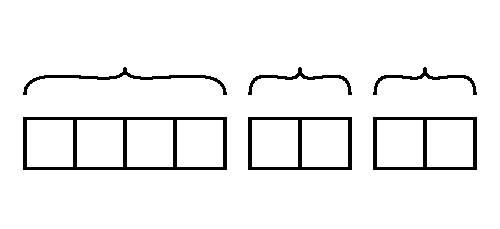
\includegraphics[scale=1]{datablock.ps}\\
   % translate x=512 y=269 scale 0.38
   \putbox{0.39in}{1.12in}{1.20}{DADOS}%
   \putbox{1.72in}{1.12in}{1.20}{SEP}%
   \putbox{2.39in}{1.12in}{1.20}{CRC16}%
   \putbox{0.22in}{0.12in}{1.20}{\centbox{\midbox{0}}}%
   \putbox{0.56in}{0.12in}{1.20}{\centbox{\midbox{1}}}%
   \putbox{0.81in}{0.12in}{1.20}{}%
   \putbox{0.89in}{0.12in}{1.20}{\centbox{\midbox{2}}}%
   \putbox{1.22in}{0.12in}{1.20}{\centbox{\midbox{3}}}%
   \putbox{1.72in}{0.12in}{1.20}{\centbox{\midbox{4}}}%
   \putbox{2.06in}{0.12in}{1.20}{\centbox{\midbox{5}}}%
   \putbox{2.56in}{0.12in}{1.20}{\centbox{\midbox{6}}}%
   \putbox{2.89in}{0.12in}{1.20}{\centbox{\midbox{7}}}%
   \putbox{1.72in}{0.46in}{0.72}{\centbox{\midbox{0xFF}}}%
   \putbox{2.06in}{0.46in}{0.72}{\centbox{\midbox{0xFF}}}%
   } % close 'parbox'
   } % close 'scalebox'
   \vspace{-\baselineskip} % this is not necessary, but looks better
\end{center}
